Minimizing with respect to $C^*_{p\alpha}$, remembering that $C^*_{p\alpha}$ and $C_{p\alpha}$ (and that the indices contain all single-particle quantum numbers including spin) are independent and defining
\begin{equation*}
    h_{\alpha\gamma}^\HF = \expval{\alpha}{h}{\gamma} + \sum_{p} \sum_{\beta\delta} C^*_{p\beta} C_{p\delta} \expval{\alpha\beta}{V}{\gamma\delta}_{AS},
\end{equation*}
show that you can write the Hartree-Fock equations as
\begin{equation*}
    \sum_{\gamma} h_{\alpha\gamma}^\HF C_{p\gamma} = \epsilon_p^{\mathrm{HF}} C_{p\alpha}. \label{eq:newhf}
\end{equation*}

Explain the meaning of the different terms and define the Hartree-Fock operator in second quantization.
Write down its diagrammatic representation as well.
The greek letters refer to the wave functions in the original basis (in our case the hydrogen-like wave functions) while roman letters refer to the new basis.

\subsection{}
We previously defined the energy functional as, using greek indices for the original basis,
\begin{equation*}
    E[\Phi] = \expval{\Phi}{\hat{H}}{\Phi} = \sum_{\alpha} \expval{\alpha}{\hat{h}_0}{\alpha} + \frac{1}{2} \sum_{\alpha\beta} \expval{\alpha\beta}{V}{\alpha \beta}_{AS}.
\end{equation*}
In the new basis, we have
\begin{equation*}
    E[\Phi^\HF] = \sum_{i} \expval{i}{\hat{h}_0}{i} + \frac{1}{2} \sum_{ij} \expval{ij}{V}{ij}_{AS}.
\end{equation*}
As $\ket{i} = \sum_{\alpha} C_{i \alpha} \ket{\alpha}$, we also have
\begin{equation*}
    \bra{i} = \ket{i}^\dagger
    = \left[ \sum_{\alpha} C_{i \alpha} \ket{\alpha} \right]^\dagger
    = \sum_{\alpha} C_{i \alpha}^* \bra{\alpha}.
\end{equation*}
This means that we can rewrite the one-body as
\begin{align*}
    \sum_i \expval{i}{\hat{h}_0}{i} = \sum_{i} \sum_{\alpha\beta} \expval{\alpha}{C_{i \alpha}^* \hat{h}_0 C_{i \beta}}{\beta} = \sum_{i} \sum_{\alpha\beta} C_{i \alpha}^* C_{i \beta}  \expval{\alpha}{\hat{h}_0}{\beta}.
\end{align*}
Similarly, we get the two-body part as
\begin{equation*}
    \frac{1}{2} \sum_{ij} \expval{ij}{V}{ij}_{AS} = \frac{1}{2} \sum_{ij} \sum_{\alpha\beta\gamma\delta} C_{i \alpha}^* C_{j \beta}^* C_{i \gamma} C_{j \delta} \expval{\alpha\beta}{V}{\gamma\delta}_{AS}.
\end{equation*}
Defining this as a functional of the coefficients $C$, we have
\begin{equation}\label{eq:E0}
    E_0[C] = \sum_{i} \sum_{\alpha\beta} C_{i \alpha}^* C_{i \beta}  \expval{\alpha}{\hat{h}_0}{\beta} + \frac{1}{2} \sum_{ij} \sum_{\alpha\beta\gamma\delta} C_{i \alpha}^* C_{j \beta}^* C_{i \gamma} C_{j \delta} \expval{\alpha\beta}{V}{\gamma\delta}_{AS}.
\end{equation}

As we are working with orthonormal basis functions, we have
\begin{equation*}
    \braket{i}{j} = \delta_{ij} = \sum_{\alpha\beta} C_{i \alpha}^* C_{i \beta} \braket{\alpha}{\beta} = \sum_{\alpha} C_{i \alpha}^* C_{i \alpha}.
\end{equation*}
With this, we define a functional $F[C]$ as
\begin{equation*}
    F[C] = E_0[C] - \sum_{i} \lambda_i \sum_{\alpha} C_{i \alpha}^* C_{i \alpha},
\end{equation*}
where $\lambda_i$ are the Lagrange multipliers enforcing the orthonormality of the basis functions.

Minimizing $F$ with respect to $C^*_{i\alpha}$, we wish to solve
\begin{equation*}
    \frac{\diff F}{\diff C^*_{i\alpha}}[C] = \frac{\diff}{\diff C_{i \alpha}^*} \left[ E_0[C] - \sum_j \lambda_j \sum_{\alpha} C_{j \alpha}^* C_{j \alpha} \right] = 0.
\end{equation*}
Considering the one-body part of $E_0$, we have
\begin{equation*}
    \frac{\diff}{\diff C_{i \alpha}^*} \sum_{i} \sum_{\alpha\beta} C_{i \alpha}^* C_{i \beta}  \expval{\alpha}{\hat{h}_0}{\beta} = \sum_{\beta} C_{i \beta} \expval{\alpha}{\hat{h}_0}{\beta}.
\end{equation*}
For the two-body part, we firstly note that $C_{i \alpha}^*$ and $C_{j \beta}^*$ of Eq.~\eqref{eq:E0} are dummy indices, meaning the factor of $1/2$ gets canceled out.
This gives us
\begin{equation*}
    \frac{\diff}{\diff C_{i \alpha}^*} \frac{1}{2} \sum_{ij} \sum_{\alpha\beta\gamma\delta} C_{i \alpha}^* C_{j \beta}^* C_{i \gamma} C_{j \delta} \expval{\alpha\beta}{V}{\gamma\delta}_{AS} = \sum_j \sum_{\beta\gamma\delta} C_{j \beta}^* C_{i \gamma} C_{j \delta} \expval{\alpha\beta}{V}{\gamma\delta}_{AS}.
\end{equation*}
For the term enforcing orthonormality, we have simply
\begin{equation*}
    \frac{\diff}{\diff C_{i \alpha}^*} \sum_{i} \lambda_i \sum_{\alpha} C_{i \alpha}^* C_{i \alpha} = \lambda_i C_{i \alpha}.
\end{equation*}
Combining these terms, we have
\begin{equation*}
    \sum_{\beta} C_{i \beta} \expval{\alpha}{\hat{h}_0}{\beta} + \sum_j \sum_{\beta\gamma\delta} C_{j \beta}^* C_{i \gamma} C_{j \delta} \expval{\alpha\beta}{V}{\gamma\delta}_{AS} - \lambda_i C_{i \alpha} = 0.
\end{equation*}
Recognizing $\lambda_i$ as the eigenvalues $\varepsilon_i^\HF$, we can rewrite this as
\begin{equation*}
    \sum_{\beta} C_{i \beta} \expval{\alpha}{\hat{h}_0}{\beta} + \sum_j \sum_{\beta\gamma\delta} C_{j \beta}^* C_{i \gamma} C_{j \delta} \expval{\alpha\beta}{V}{\gamma\delta}_{AS} = \varepsilon_i^\HF C_{i \alpha}.
\end{equation*}

Changing the label of the dummy variables $\beta \mapsto \gamma$ in the one-body term and $i \mapsto p$ everywhere, we can write this as
\begin{gather*}
    \sum_{\gamma} C_{p \gamma} \expval{\alpha}{\hat{h}_0}{\gamma} + \sum_j \sum_{\beta\gamma\delta} C_{j \beta}^* C_{p \gamma} C_{j \delta} \expval{\alpha\beta}{V}{\gamma\delta}_{AS} = \varepsilon_p^\HF C_{p \alpha} \\
    \sum_{\gamma} C_{p \gamma} \left[ \expval{\alpha}{\hat{h}_0}{\gamma} + \sum_j \sum_{\beta\delta} C_{j \beta}^*  C_{j \delta} \expval{\alpha\beta}{V}{\gamma\delta}_{AS} \right] = \varepsilon_p^\HF C_{p \alpha} \\
    \sum_{\gamma} h_{\alpha\gamma}^\HF C_{p \gamma} = \varepsilon_p^\HF C_{p \alpha},
\end{gather*}
as we wanted to show, where $\varepsilon_p^\HF$ are the new single-particle energies we solve for.

Using the density matrix, defined by
\begin{equation*}
    \rho_{\beta\delta} = \sum_{i} \braket{\beta}{i} \braket{i}{\delta} = \sum_{i} C_{i\beta} C_{i\delta}^*,
\end{equation*}
we can write $h_{\alpha \gamma}^\HF$ as
\begin{equation*}
    h_{\alpha \gamma}^\HF = \expval{\alpha}{\hat{h}_0}{\gamma} + \sum_{\beta\delta} \rho_{\beta\delta} \expval{\alpha\beta}{V}{\gamma\delta}_{AS}.
\end{equation*}

In second quantization with respect to the old basis, the Hartree-Fock operator is then defined as
% \begin{equation*}
%     \hat{h}^\HF = \sum_{\alpha\gamma} h_{\alpha\gamma}^\HF a_\alpha^\dagger a_\gamma.
% \end{equation*}
\begin{equation*}
    \hat{h}^\HF = \sum_{\alpha \gamma} \hat{h}^\HF_{\alpha\gamma} a_\alpha^\dagger a_\gamma = \sum_{\alpha \gamma} \expval{\alpha}{\hat{h}^\HF}{\gamma} a_\alpha^\dagger a_\gamma
\end{equation*}

We are then interested in the second quantized form with respect to the new basis, namely
\begin{equation*}
    \hat{h}^\HF = \sum_{pq} \hat{h}^\HF_{p q} a_p^\dagger a_q.
\end{equation*}
We have
\begin{align*}
    \hat{h}^\HF_{p q} &= \expval{p}{\hat{h}^\HF}{q} \\
    &= \sum_{\alpha \beta} C_{p \alpha}^* \expval{\alpha}{\hat{h}^\HF}{\beta} C_{q \beta} \\
    &= \sum_{\alpha\gamma} C_{p\alpha}^* \left[ \expval{\alpha}{\hat{h}_0}{\gamma} + \sum_{\beta\delta} \rho_{\beta\delta} \expval{\alpha\beta}{V}{\gamma\delta}_{AS} \right] C_{q\gamma} \\
    &= \sum_{\alpha\gamma} C_{p\alpha}^* \expval{\alpha}{\hat{h}_0}{\gamma} C_{q\gamma} + \sum_{\alpha\gamma} C_{p\alpha}^* \sum_{\beta\delta} \rho_{\beta\delta} \expval{\alpha\beta}{V}{\gamma\delta}_{AS} C_{q\gamma} \\
    &= \expval{p}{\hat{h}_0}{q} + \sum_{i} \expval{p i }{V}{q i}_{AS}.
\end{align*}
This gives us the second quantized form of the Hartree-Fock operator as
\begin{equation*}
    \hat{h}^\HF = \sum_{pq} \left[ \expval{p}{\hat{h}_0}{q} + \sum_{i} \expval{pi}{V}{qi}_{AS} \right] a_p^\dagger a_q.
\end{equation*}

For the diagrammatic representation, we only consider the cases $\expval{i}{h^\HF}{i}$ and $\expval{a}{h^\HF}{a}$, as the other cases vanish.
This gives us the diagram shown in Fig.~\ref{fig:HF-diagram}.

\begin{figure}[ht]
    \centering
    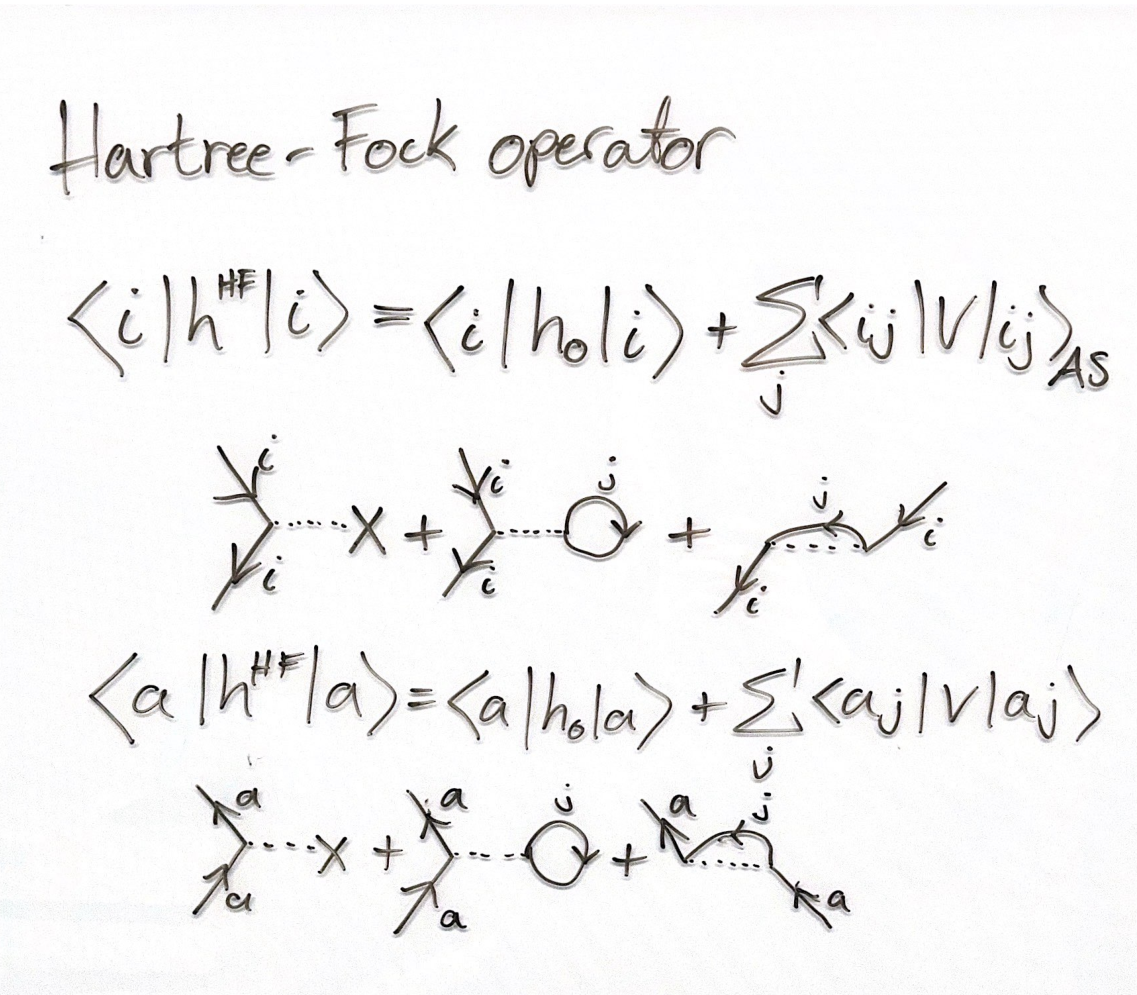
\includegraphics[width=0.5\textwidth]{figs/HF-operator.pdf}
    \caption{Diagrammatic representation of $\expval{i}{h^\HF}{i}$ and $\expval{a}{h^\HF}{a}$.\label{fig:HF-diagram}}
\end{figure}
